% Options for packages loaded elsewhere
\PassOptionsToPackage{unicode}{hyperref}
\PassOptionsToPackage{hyphens}{url}
%
\documentclass[
]{article}
\usepackage{amsmath,amssymb}
\usepackage{iftex}
\ifPDFTeX
  \usepackage[T1]{fontenc}
  \usepackage[utf8]{inputenc}
  \usepackage{textcomp} % provide euro and other symbols
\else % if luatex or xetex
  \usepackage{unicode-math} % this also loads fontspec
  \defaultfontfeatures{Scale=MatchLowercase}
  \defaultfontfeatures[\rmfamily]{Ligatures=TeX,Scale=1}
\fi
\usepackage{lmodern}
\ifPDFTeX\else
  % xetex/luatex font selection
\fi
% Use upquote if available, for straight quotes in verbatim environments
\IfFileExists{upquote.sty}{\usepackage{upquote}}{}
\IfFileExists{microtype.sty}{% use microtype if available
  \usepackage[]{microtype}
  \UseMicrotypeSet[protrusion]{basicmath} % disable protrusion for tt fonts
}{}
\makeatletter
\@ifundefined{KOMAClassName}{% if non-KOMA class
  \IfFileExists{parskip.sty}{%
    \usepackage{parskip}
  }{% else
    \setlength{\parindent}{0pt}
    \setlength{\parskip}{6pt plus 2pt minus 1pt}}
}{% if KOMA class
  \KOMAoptions{parskip=half}}
\makeatother
\usepackage{xcolor}
\usepackage[margin=1in]{geometry}
\usepackage{graphicx}
\makeatletter
\def\maxwidth{\ifdim\Gin@nat@width>\linewidth\linewidth\else\Gin@nat@width\fi}
\def\maxheight{\ifdim\Gin@nat@height>\textheight\textheight\else\Gin@nat@height\fi}
\makeatother
% Scale images if necessary, so that they will not overflow the page
% margins by default, and it is still possible to overwrite the defaults
% using explicit options in \includegraphics[width, height, ...]{}
\setkeys{Gin}{width=\maxwidth,height=\maxheight,keepaspectratio}
% Set default figure placement to htbp
\makeatletter
\def\fps@figure{htbp}
\makeatother
\setlength{\emergencystretch}{3em} % prevent overfull lines
\providecommand{\tightlist}{%
  \setlength{\itemsep}{0pt}\setlength{\parskip}{0pt}}
\setcounter{secnumdepth}{5}
\usepackage[german]{babel}
\usepackage{mathtools}
\usepackage{tikz}
\usepackage{pgf}
\usepackage{csquotes}
\AtBeginDocument{
\renewcommand{\maketitle}{}
}
\PassOptionsToPackage{a4paper,margin = 2.5cm}{geometry}
\usepackage{geometry}
\newcommand{\bcenter}{\begin{center}}
\newcommand{\ecenter}{\end{center}}
\renewcommand{\contentsname}{Inhalt}
\usepackage{blindtext}
\usepackage[backend=biber, style = apa]{biblatex}
\addbibresource{Literatur.bib}
\usepackage{multirow}
\usepackage{booktabs}
\usepackage{array}
\usepackage{pdflscape}
\usepackage{afterpage}
\ifLuaTeX
  \usepackage{selnolig}  % disable illegal ligatures
\fi
\usepackage[]{biblatex}
\addbibresource{Literatur.bib}
\usepackage{bookmark}
\IfFileExists{xurl.sty}{\usepackage{xurl}}{} % add URL line breaks if available
\urlstyle{same}
\hypersetup{
  pdftitle={Ergebnisse},
  pdfauthor={Franz Andersch \& Niklas Münz},
  hidelinks,
  pdfcreator={LaTeX via pandoc}}

\title{Ergebnisse}
\author{Franz Andersch \& Niklas Münz}
\date{2024-08-26}

\begin{document}
\maketitle

\subsection{Vorgehensweise bei der Analyse}

Bevor die Ergebnisse erläutert werden, wird kurz auf die Vorgehensweise
bei der Analyse eingegangen. In die Analyse werden fünf Modelle
einbezogen: SVM mit linearem, polynomialem und radialem Kern, sowie
regularisierte logistische Regression und k-nearest neighbours.\newline
Vor dem erstellen der Modelle wird ein Tuning der Hyperparameter je
Modell durchgeführt. Dafür wird die Bayesian Optimization Methode
genutzt, welche ein iterativer Algorithmus ist. Hierbei werden die
nächsten Evaluierungspunkte basierend auf zuvor beobachteten Ergebnissen
bestimmt \parencite{yangHyperparameterOptimizationMachine2020}. Der
Algorithmus basiert auf zwei Hauptkomponenten: einem Surrogatmodell und
einer Akqusitionsfunktion. Das Surrogatmodell, wofür hier ein Gaussian
Process genutzt wird, passt die bisher beobachteten Punkte an die
Zielfunktion an. Die Akquisitionsfunktion wählt dann die nächsten Punkte
aus, wobei ein Gleichgewicht zwischen der Erkundung neuer Bereiche und
der Nutzung vielversprechender Regionen angestrebt wird. Dafür wird hier
der Ansatz des Upper-Confidence-Bound genutzt, welcher obere
Konfidenzgrenzen nutzt um den Verlust gegenüber der besten möglichen
Entscheidung, während der Optimierung zu minimieren
\parencite{snoekPracticalBayesianOptimization2012}. \begin{align}
a_{UCB}(\mathbf{x};~\left\{\mathbf{x}_n,y_n\right\},\theta) = \mu(\mathbf{x};~\left\{\mathbf{x}_n,y_n\right\},\theta) + k \sigma(\mathbf{x};~\left\{\mathbf{x}_n,y_n\right\},\theta)
\end{align} Die Bayesian Optimization wird genutzt, da sie eine schnelle
Konvergenz für stetige Hyperparameter aufweist
\parencite{yangHyperparameterOptimizationMachine2020}. Als
Evaluierungskriterium wird die Genauigkeit der Modelle, welche durch den
Anteil der korrekt klassifizierten Beobachtungen wiedergegeben wird,
verwendet. Zur Bestimmung dieser werden die erzeugten Testdaten
herangezogen.

Basierend auf den Ergebnissen des Tuning werden die oben genannten
Modelle erstellt. Daraufhin werden die Genauigkeit, die Receiver
Operating Characteristic Kurve (ROC-Kurve) bzw. der Area Under The Curve
Wert (AUC-Wert) und der F1-Score für jedes Modell bestimmt.\newline Die
ROC-Kurve ist eine grafische Darstellung der Leistungsfähigkeit eines
Klassifikationsmodells, wobei die Sensitivität auf der y-Achse von 0 bis
1 gegen die Spezifität auf der x-Achse von 1 bis 0 abgetragen wird
\parencite{fawcettIntroductionROCAnalysis2006}. Sensitivität und
Spezifität ergeben sich aus: \begin{align}
Sensitivität=\frac{korrekt~Positiv}{korrekt~Positiv~+~falsch~Negativ}
\end{align} \begin{align}
Spezifität=\frac{korrekt~Negativ}{falsch~Positiv~+~korrekt~Negativ}
\end{align} Positiv ist in diesem Fall gleichbedeutend mit Klasse 1 und
Negativ mit Klasse 2. Die ROC-Kurve zeigt dann den Zusammenhang zwischen
dem Nutzen (korrekt Positive) und den Kosten (falsch Positive) auf. Eine
ideale Kurve läuft nah am linken, oberen Rand der Grafik, da hier
bereits bei sehr hoher Spezifität (hohe Anzahl korrekt Negative) eine
hohe Sensitivität (hohe Anzahl korrekt Positive) erreicht wird. Der
AUC-Wert bezieht sich auf die Fläche unterhalb der Kurve und liegt somit
im Intervall {[}0,1{]}, wobei ein Wert von 1 für eine perfekte
Klassifikation spricht, während ein Wert von 0.5 glechbedeutend mit
einer rein zufälligen Zuordnung der Klassen spricht.\newline Für den
F1-Score ist außerdem die Präzision von Bedeutung, die sich wie folgt
berechnet\parencite{fawcettIntroductionROCAnalysis2006}: \begin{align}
Präzision=\frac{korrekt~Positiv}{korrekt~Positiv~+~falsch~Positiv}
\end{align} Der F1-Score beschreibt das harmonische Mittel zwischen
Präzision und Sensitivität und drückt folglich die Fähigkeit des
Modells, gleichzeitig falsch Positive und falsch Negative zu minimieren,
aus. \begin{align}
F1\text{-}Score=\frac{2}{1/Präzision~+~1/Sensitivität}
\end{align}\newline Zuletzt wird innerhalb jeder Datensituation, für
jeden Algorithmus ein Rang vergeben, der sich aus der Summe der drei
Auswertungskriterien Genauigkeit, AUC-Wert sowie F1-Score ergibt. Dabei
steht Rang 1 für den am besten abschneidenden Algorithmus in der
jeweiligen Datensituation.

\subsection{Darstellung der Ergebnisse}

Tabelle \ref{tab:TabVergleich} zeigt die Leistungsfähigkeit der fünf
Klassifikationsalgorithmen über die neun verschiedenen Datensituationen
anhand drei verschiedener Evaluationskriterien, sowie den Rang in der
jeweiligen Datensituation.\newline \afterpage{
\clearpage
\begin{landscape}

\begin{table}[h] \centering \begin{tabular}{|c|c|c|c|} \hline
 & \textbf{linear} & \textbf{polynomial} & \textbf{radial} \\ \hline \multirow{5}{*}{\textbf{$p \ll n$}} &  
\begin{tabular}{lrrrr}
\toprule
  & ACC & AUC & F1 & Rang\\
\midrule
SVM-L & 0.964 & 0.991 & 0.964 & 2\\
SVM-P & 0.964 & 0.991 & 0.964 & 2\\
SVM-R & 0.961 & 0.990 & 0.961 & 4\\
LogR & 0.965 & 0.991 & 0.965 & 1\\
K-NN & 0.571 & 0.600 & 0.567 & 5\\
\bottomrule
\end{tabular}  &  
\begin{tabular}{lrrrr}
\toprule
  & ACC & AUC & F1 & Rang\\
\midrule
SVM-L & 0.759 & 0.802 & 0.752 & 4\\
SVM-P & 0.764 & 0.802 & 0.756 & 2\\
SVM-R & 0.904 & 0.972 & 0.904 & 1\\
LogR & 0.762 & 0.802 & 0.751 & 3\\
K-NN & 0.756 & 0.800 & 0.756 & 5\\
\bottomrule
\end{tabular}  &  
\begin{tabular}{lrrrr}
\toprule
  & ACC & AUC & F1 & Rang\\
\midrule
SVM-L & 0.497 & 0.495 & 0.504 & 5\\
SVM-P & 0.926 & 0.981 & 0.926 & 1\\
SVM-R & 0.792 & 0.888 & 0.801 & 2\\
LogR & 0.500 & 0.500 & 0.667 & 4\\
K-NN & 0.687 & 0.749 & 0.657 & 3\\
\bottomrule
\end{tabular}  \\ \hline \multirow{5}{*}{\textbf{$p \approx n$}} &  
\begin{tabular}{lrrrr}
\toprule
  & ACC & AUC & F1 & Rang\\
\midrule
SVM-L & 0.80 & 0.851 & 0.783 & 3\\
SVM-P & 0.80 & 0.851 & 0.783 & 3\\
SVM-R & 0.86 & 0.885 & 0.851 & 1\\
LogR & 0.80 & 0.858 & 0.783 & 2\\
K-NN & 0.70 & 0.698 & 0.681 & 5\\
\bottomrule
\end{tabular}  &  
\begin{tabular}{lrrrr}
\toprule
  & ACC & AUC & F1 & Rang\\
\midrule
SVM-L & 0.60 & 0.590 & 0.524 & 3\\
SVM-P & 0.60 & 0.590 & 0.524 & 3\\
SVM-R & 0.60 & 0.586 & 0.545 & 2\\
LogR & 0.56 & 0.437 & 0.500 & 5\\
K-NN & 0.62 & 0.729 & 0.642 & 1\\
\bottomrule
\end{tabular}  &  
\begin{tabular}{lrrrr}
\toprule
  & ACC & AUC & F1 & Rang\\
\midrule
SVM-L & 0.58 & 0.531 & 0.462 & 5\\
SVM-P & 0.84 & 0.830 & 0.826 & 1\\
SVM-R & 0.74 & 0.889 & 0.794 & 2\\
LogR & 0.58 & 0.699 & 0.364 & 4\\
K-NN & 0.80 & 0.800 & 0.762 & 3\\
\bottomrule
\end{tabular}  \\ \hline \multirow{5}{*}{\textbf{$p \gg n$}} &  
\begin{tabular}{lrrrr}
\toprule
  & ACC & AUC & F1 & Rang\\
\midrule
SVM-L & 0.66 & 0.725 & 0.653 & 4\\
SVM-P & 0.70 & 0.750 & 0.681 & 3\\
SVM-R & 0.64 & 0.500 & 0.609 & 5\\
LogR & 0.72 & 0.754 & 0.741 & 2\\
K-NN & 0.80 & 0.866 & 0.808 & 1\\
\bottomrule
\end{tabular}  &  
\begin{tabular}{lrrrr}
\toprule
  & ACC & AUC & F1 & Rang\\
\midrule
SVM-L & 0.48 & 0.485 & 0.480 & 4\\
SVM-P & 0.50 & 0.517 & NaN & 5\\
SVM-R & 0.56 & 0.500 & 0.450 & 3\\
LogR & 0.64 & 0.642 & 0.654 & 2\\
K-NN & 0.70 & 0.700 & 0.706 & 1\\
\bottomrule
\end{tabular}  &  
\begin{tabular}{lrrrr}
\toprule
  & ACC & AUC & F1 & Rang\\
\midrule
SVM-L & 0.50 & 0.570 & 0.390 & 4\\
SVM-P & 0.76 & 0.726 & 0.750 & 1\\
SVM-R & 0.66 & 0.757 & 0.738 & 3\\
LogR & 0.54 & 0.538 & 0.343 & 5\\
K-NN & 0.76 & 0.760 & 0.700 & 2\\
\bottomrule
\end{tabular}  \\ \hline \end{tabular} \caption{Vergleich der Modelle} \label{tab:TabVergleich} \end{table}

\end{landscape}
\clearpage
} \textless\textless\textless\textless\textless\textless\textless{} HEAD
In den Datensituationen mit linearer Form der Entscheidungsgrenze
performt insbesondere \textit{logR} gut, da sie in allen drei Szenarien
über alle Kriterien hinweg einen Wert von mindestens 0.72 aufweist und
jeweils mindestens Rang 2 belegt. Im Falle von \(p \ll n\) und
\(p \approx n\) zeigen auch \textit{SVM-L}, \textit{SVM-P} und
\textit{SVM-R} eine gute Leistung mit Werten nahe 0.9 bzw. 0.8. In dem
hochdimensionalen Setting \(p \gg n\) schneiden alle Drei, jedoch
insbesondere \textit{SVM-R} schlechter ab, welche einen AUC-Wert von 0.5
aufweist. \textit{K-NN} schneidet im linearen Kontext für \(p \ll n\)
und \(p \approx n\) am schlechtesten ab, wobei der Unterschied im
niedrigdimensionalen Raum am deutlichsten ist (0.39 schlechtere
Genauigkeit als der nächst schlechteste Algorithmus). Im
hochdimensionalen Raum kann \textit{K-NN} allerdings als bester
Algorithmus mit Werten über 0.8 überzeugen.\newline Die ROC-Kurven
werden nur in den Datensituationen mit \(p \ll n\) genutzt, da die
grafische Darstellung in Szenarien mit kleinem \(n\) nicht sinnvoll
erscheint. Es ist dazu zu sagen, das SVM anders als beispielsweise
logistische Regression, nicht direkt eine Wahrscheinlichkeit ausgeben,
dass eine Beobachtung zu einer bestimmten Klasse gehört. Da diese
Wahrscheinlichkeit aber für die ROC-Kurven benötigt wird, gibt es auch
hier Möglichkeiten diese für die SVM zu berechnen (siehe
\cite{plattProbabilisticOutputsSupport2000}). Abbildung \ref{fig:S1ROC}
zeigt die ROC-Kurven für die Datensituation S1. Diese zeigt grafisch
noch einmal den deutlichen Unterschied zwischen \textit{K-NN}, welcher
nur etwas besser als eine reine Zufallsauswahl ist und den anderen vier
Algorithmen, welche nahezu perfekt klassifizieren.

In den Datensituationen mit polynomialer Form der Entscheidungsgrenze
ist die Leistungsfähigkeit aller Algorithmen grundsätzlich schlechter
als in den zuvor beschriebenen Szenarien. Im Fall von \(p \ll n\) sind
die Ergebnisse ausschließlich für \textit{SVM-R} sehr gut mit Werten
über 0.9. Die restlichen Algorithmen performen mittelmäßig mit Werten um
0.7, wobei sich hier kein Algorithmus von den anderen absetzen kann. Bei
\(p \approx n\) ist \textit{K-NN} den anderen Klassifikationsmethoden
leicht überlegen, insbesondere beim AUC-Wert mit 0.729. Die anderen
Algorithmen befinden sich durchweg über alle Werte hinweg nahe 0.5.
Ähnlich ist es der Fall für \(p \gg n\) bei dem auch wieder
\textit{K-NN} eine leicht bessere Leistung zeigt mit einer Genauigkeit
von 0.7, gefolgt von \textit{LogR} mit 0.64. Dennoch ist für die letzten
beiden Szenarien deutlich, dass kein Algorithmus gute Leistung
zeigt.\newline Abbildung \ref{fig:S2ROC} zeigt die ROC-Kurven für
Szenario 2. Hier ist gut ersichtlich, dass sich \textit{SVM-R} von den
anderen Algorithmen abheben kann, welche alle eine mittelmäßige Leistung
zeigen.

In den Datensituationen mit radialer Form der Entscheidungsgrenze ist
für den Fall \(p \ll n\) eine eindeutige Unterscheidung zu treffen.
Während \textit{SVM-P}, \textit{SVM-R} und \textit{K-NN} gut
klassifizieren, haben dabei \textit{SVM-L} und \textit{LogR} große
Probleme und zeigen lediglich Werte nahe 0.5. Insbesondere
\textit{SVM-P} zeigt mit einem AUC-Wert von 0.981 eine sehr gute
Performance. Weniger drastisch aber dennoch mit dem gleichen Resultat
ist dies für \(p \approx n\) der Fall. Während \textit{SVM-P} etwas
schlechter performt, bleibt \textit{SVM-R} nahezu identisch und
\textit{K-NN} kann sich sogar leicht steigern auf einen AUC-Wert von
0.8. \textit{SVM-L} und \textit{LogR} können sich leicht verbessern
(beispielsweise mit einer Genauigkeit nahe 0.6). Für \(p \gg n\) sind
ebenfalls die beiden Gruppen zu differenzieren. Für \textit{SVM-L} und
\textit{LogR} sind wie in Szenario 3 wieder Werte nahe 0.5 für die
Genauigkeit erkennbar. \textit{SVM-P} und \textit{K-NN} performen in
diesem Szenario am Besten. \textit{SVM-R} fällt insbesondere mit einer
Genauigkeit von 0.66 im Vergleich zu 0.76 etwas hinter den anderen
beiden Algorithmen zurück.\newline Abbildung \ref{fig:S3ROC} zeigt die
ROC-Kurven für Szenario 3. Hieraus wird einerseits die Aufteilung in die
zwei Gruppen deutlich. \textit{SVM-P}, \textit{SVM-R} und \textit{K-NN}
bewegen sich näher an der oberen linken Kante, was für eine (nahezu)
perfekte Klassifikation spricht. Andererseits ist eindeutig, dass sich
\textit{SVM-P} nochmal von den anderen beiden Algorithmen absetzen kann.
\textit{SVM-L} und \textit{LogR} orientieren sich nahe der diagonalen
Linie, die eine ROC-Kurve einer reinen Zufallsauswahl beschreibt. Dies
zeigt auf, dass sie kaum Fähigkeit aufweisen zwischen den Klassen zu
unterscheiden.

\begin{figure}[htb]
\begin{minipage}{0.48\linewidth}
\centering
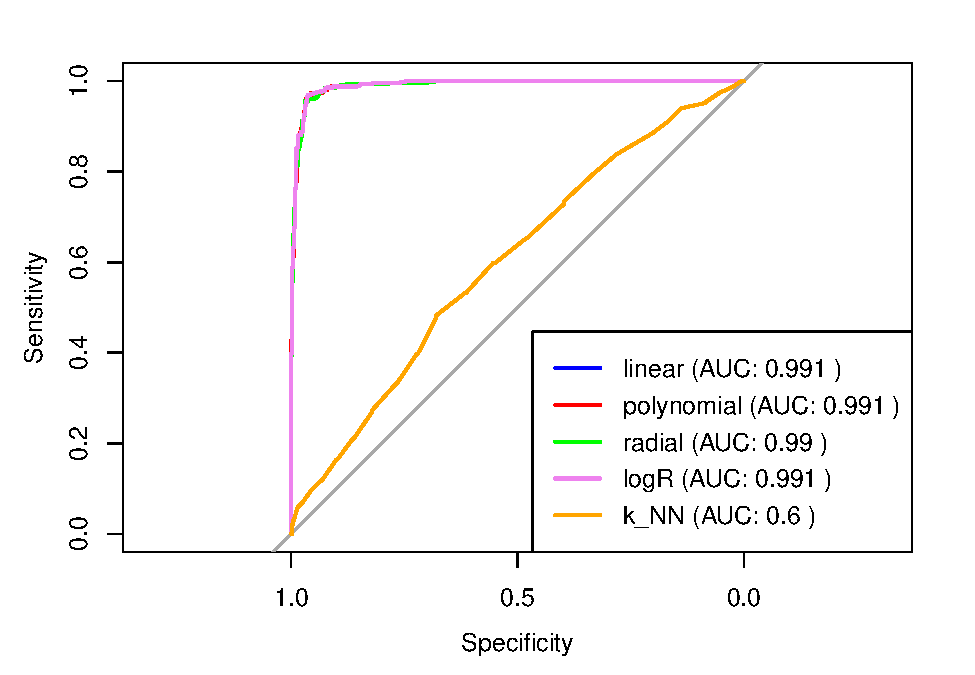
\includegraphics{Ergebnisse_files/figure-latex/S1ROC-1.pdf}
\caption{ROC-Kurven Szenario 1}
\label{fig:S1ROC}
\end{minipage}
\hfill
\begin{minipage}{0.48\linewidth}
\centering
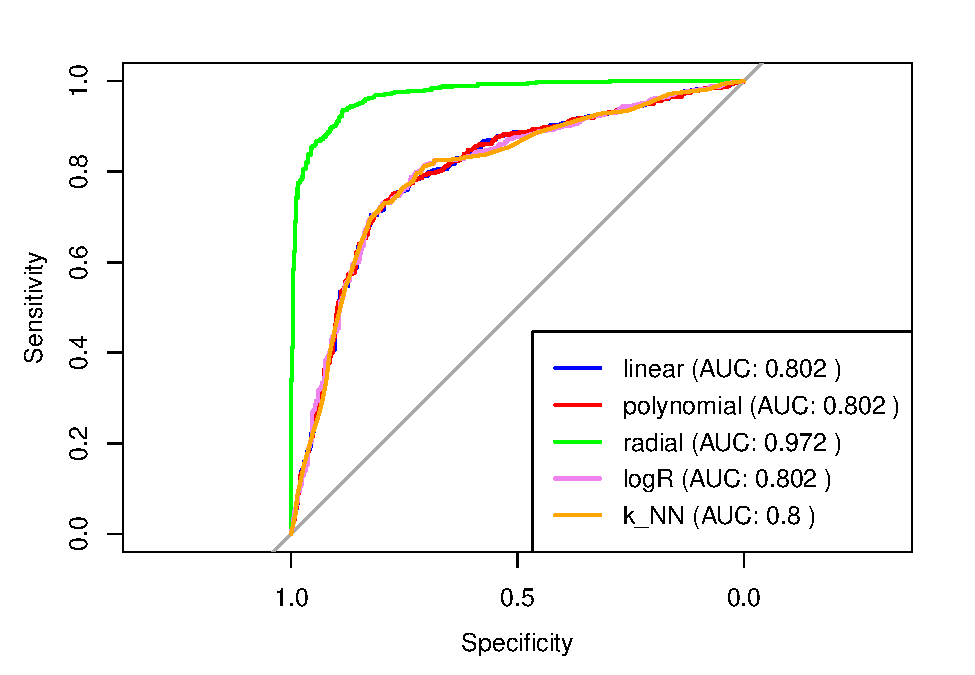
\includegraphics{Ergebnisse_files/figure-latex/S2ROC-1.pdf}
\caption{ROC-Kurven Szenario 2}
\label{fig:S2ROC}
\end{minipage}
\vspace*{0.5cm}\newline
\begin{minipage}{\linewidth}
\centering
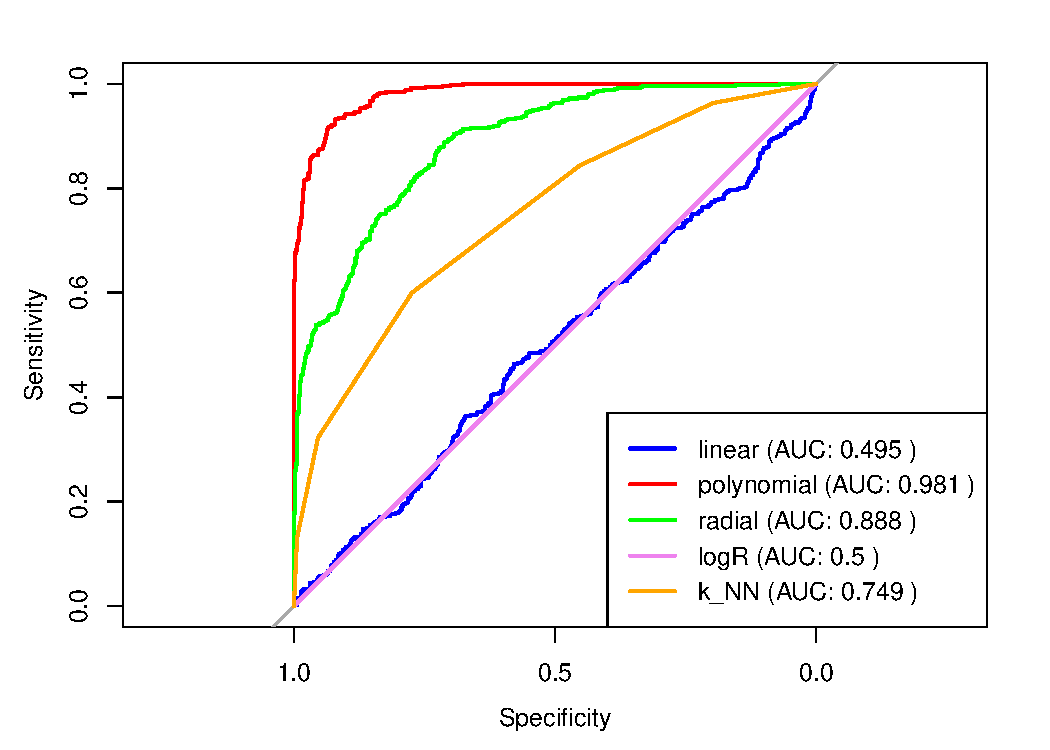
\includegraphics[width=0.48\linewidth]{Ergebnisse_files/figure-latex/S3ROC-1.pdf}
\caption{ROC-Kurven Szenario 3}
\label{fig:S3ROC}
\end{minipage}
\end{figure}

Zuletzt wird ein Vergleich der einzelnen Dimensionen über die drei
Formen der Entscheidungsgrenze gezogen. So ist für \(p \ll n\)
ersichtlich, dass insbesondere \textit{SVM-P} und \textit{SVM-R} über
alle drei Szenarien gute Leistung (mit Werten mindestens nahe 0.8 über
alle drei Szenarien) zeigen. Ähnliches gilt, mit Ausnahme der
polynomialen Form der Entscheidungsgrenze, auch für \(p \approx n\),
wobei hier auch \textit{K-NN} gute Werte zeigt (alle drei durchweg mit
Werten über 0.7). In den hochdimensionalen Szenarien \(p \gg n\) ist
einzig \textit{K-NN} überzeugend, welcher auch im polynomialen Szenario
Werte über 0.7 aufweist.

\printbibliography

\end{document}
